	\documentclass[10pt,oneside]{CBFT_book}
	% Algunos paquetes
	\usepackage{amssymb}
	\usepackage{amsmath}
	\usepackage{graphicx}
	\usepackage{libertine}
% 	\usepackage[bold-style=TeX]{unicode-math}
	\usepackage{lipsum}

	\usepackage{natbib}
	\setcitestyle{square}

	\usepackage{polyglossia}
	\setdefaultlanguage{spanish}


	\usepackage{CBFT.estilo} % Cargo la hoja de estilo
	
	% Tipografías
	% \setromanfont[Mapping=tex-text]{Linux Libertine O}
	% \setsansfont[Mapping=tex-text]{DejaVu Sans}
	% \setmonofont[Mapping=tex-text]{DejaVu Sans Mono}

	%===================================================================
	%	DOCUMENTO PROPIAMENTE DICHO
	%===================================================================

% \title{CBFT Mecánica clásica}
% \author{Fuerzas centrales}
% \date{\today}

\begin{document}
% \maketitle
% \tableofcontents

\chapter{Fuerzas centrales}

% =================================================================================================
\section{Fuerzas centrales}\index{Fuerzas centrales}
% =================================================================================================

\notamargen{Comentario de que fijo un punto, y es una función vectorial tomar vector y da vector, que resulta finalmente
más simple porque se sabe de antemano la dirección de la salida --en la dirección de la recta que une los puntos--.}

Una fuerza central es aquella que depende únicamente de la distancia entre dos puntos. Es decir que si se tienen dos
puntos $\vb{x}, \vb{y}$, separados una distancia $ r = |\vb{r}| = |\vb{x} - \vb{y}| $, una fuerza central $\vb{F}$ verifica
\[
	\vb{F}( \vb{x}, \vb{y} ) = F(r) \: \hat{r}, \qquad \qquad \hat{r} = \frac{\vb{r}}{r}
\]
% es decir que la fuerza $\vb{F}$ entre dos puntos $\vb{x}, \vb{y}$ depende de la distancia $r = |\vb{x}-\vb{y}|$
% entre los mismos.
de manera que la información sobre la dirección de la misma ($\hat{r}$) está establecida en la recta que une $\vb{x}$ con 
$\vb{y}$ mientras que su módulo es una función escalar $F(r)$.


\begin{figure}[!hbt]
	\begin{center}
	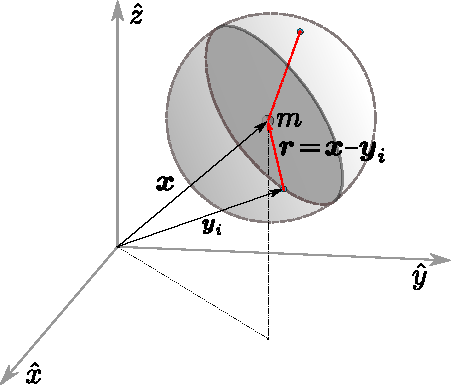
\includegraphics[width=0.4\textwidth]{images/fig_fuerza_central.pdf}	 
	\end{center}
	\caption{}
\end{figure} 

Esto implica, al ser una fuerza dependiente de una sola coordenada, que siempre es posible obtener un potencial
a partir de ella, es decir que existe $V(r)$ tal que
\[
	F(r) = - \dpar{V}{r}.
\]
\notamargen{Hay que elaborar bastante aquí: la fuerza central implica la simetría esférica porque tomado como origen
de coordenadas uno de los dos puntos $\vb{x}$ o $\vb{y}$, la fuerza por otro punto que se halle a la misma distancia
$r$ tendrá la misma magnitud. Además, el torque de la fuerza respecto a ese origen será nulo puesto que son paralelos
$\vb{r}$ y $\vb{F}$. Anoté en la carpeta: el lagrangiano es un potencial de superficies equipotenciales esféricas, entonces
se conserva el momento angular.}

Entonces, para una partícula libre el lagrangiano se puede escribir en coordenadas esféricas $(r,\theta,\phi)$ como
\[
	\Lag = \frac{1}{2}m \left( \dot{r}^2 + r^2 \dot{\theta}^2 + r^2 \sin(\theta)^2\dot{\phi}^2 \right)
\]

El momento angular $\vb{L}$ se conserva puesto que $\vb{\tau} = \vb{x} \times \vb{F}=0$. Como es 
$\vb{L} = \vb{x} \times \vb{p} = \vb{x} \times m \: \dot{\vb{x}} = cte$ entonces se sigue que $\vb{r},\vb{p}$
se hallan contenidos en el mismo plano.

Puedo pedir, sin pérdida de generalidad, que $\theta=\pi/2$ (se sitúa la partícula en el plano $xy$) y entonces
se tienen dos grados de libertad,
\[
	\Lag = \frac{1}{2}m \left( \dot{r}^2 + r^2 \dot{\theta}^2 \right) - V(r).
\]

Como $\phi$ es cíclica se tiene
\be
	\dpar{\Lag}{\dot{\phi}} = L = mr^2\dot{\phi}
	\label{ec_mov_uno}
\ee
que no es otra cosa que la conservación del momento angular (la primera ecuación de movimiento). Esa información puede 
ser llevada al lagrangiano,
\be
	\Lag = \frac{1}{2}m \dot{r}^2 + \left[ \frac{L^2}{2 m r^2} - V(r) \right]
	\label{lag_pot_central}
\ee
donde el último corchete será lo que llamaremos un potencial efectivo\footnote{Debido a la conservación del momento 
angular la parte de la energía dependiente de $\phi$, o mejor dicho debida a la rotación en $\phi$ se ha podido 
expresar en términos de $r$; entonces pasa a formar parte del potencial.}\index{potencial efectivo} $V_{\text{eff}}$, y 
el lagrangiano adopta la forma
\[
	\Lag = \frac{1}{2}m \dot{r}^2 + V_{\text{eff}}(r).
\]
Digamos que el potencial efectivo sería todos aquellos términos que no tienen la forma de la energía cinética 
(cuadrática en velocidades).
Notemos que ahora el lagrangiano depende solamente de $r$; el problema ha resulado para un único grado de libertad.

Dado el sistema elegido (movimiento plano en $xy$) ahora el $p_\phi$ es el $L$ total; en cambio, de haber elegido otro 
plano el $p_\phi$ sería el $L_z$.

La ecuación de Euler-Lagrange para el lagrangiano \eqref{lag_pot_central} resulta en
\[
	m\ddot{r} - \frac{L^2}{mr^3} + \dpar{V}{r} = 0.
\]
Integrando esta ecuación se llega a la conservación de la energía pero podemos utilizar el hecho de saber que la 
misma se conserva y escribir su expresión explícita
\be
	E = T - V = \frac{1}{2}m \dot{r}^2 + \frac{L^2}{2 m r^2} + V(r).
	\label{ec_mov_dos}
\ee

A partir de estas constantes $L,E$ tengo dos ecuaciones de primer orden \eqref{ec_mov_uno} y \eqref{ec_mov_dos}. Se han 
podido {\it ahorrar} dos integraciones: la integral de $\ddot{r}$ para obtener $\dot{r}$ y la integral de $\ddot{\phi}$ 
para hallar $\dot{\phi}$.

Desde la ecuación \eqref{ec_mov_dos} se puede integrar directamente la trayectoria $r=r(t)$ según
\[
	\dtot{r}{t} = \sqrt{ \frac{2}{m}\left( E - \frac{L^2}{2 m r^2} - V(r) \right)},
\]
o bien 
\[
	\int_{t_i}^{t_f} dt = \int_{r(t_i)}^{r(t_f)} \frac{dr}{\sqrt{\frac 2 m ( E - \frac{L^2}{2 m r^2} - V(r) )}},
\]
integral que en principio siempre tiene solución.
A partir de la ecuación \eqref{ec_mov_uno} se puede obtener la trayectoria en el espacio físico $r=r(\phi)$, o 
equivalentemente $\phi=\phi(r)$.
\[
	\dtot{\phi}{t} = \dtot{\phi}{r} \dot{r} =  \frac{L}{mr^2} 
\]
e incorporando de la \eqref{ec_mov_dos} la expresión de $\dot{r}$ se puede llegar a 
\[
	\int_{\phi_i}^{\phi_f} d\phi = \int_{r(\phi_i)}^{r(\phi_f)} 
	\frac{L}{\sqrt{ 2 m r^4 \left( E - \frac{L^2}{2 m r^2} - V(r) \right)}}dr
\]
y la resolución total del problema dependerá de la forma $V(r)$.
\notamargen{Embellecer un poco las expresiones por el aspecto odd de las raíces y todo eso.}

Consideremos, para fijar ideas, un potencial general del tipo 
\[
	V(r)  = \alpha r^{-n} 
\]
que es un potencial cuyo comportamiento dependerá del signo de la constante que acompaña. Los casos posibles serán 
\[
	\alpha = \begin{cases}
	\alpha > 0 \qquad \text{ potencial repulsivo} \\
	\alpha = 0 \qquad \text{ partícula libre} \\
	\alpha > 0 \qquad \text{ potencial repulsivo} 
	\end{cases}
\]
En un gŕafico de potencial y energía en función del radio se pueden analizar muchos aspectos de la física bajo ese 
potencial (como se hizo en el ejemplo XX del capítulo XX)

Para el caso de $\alpha > 0$ se tiene una situación como la que se ilustra en la figura bajo estas líneas
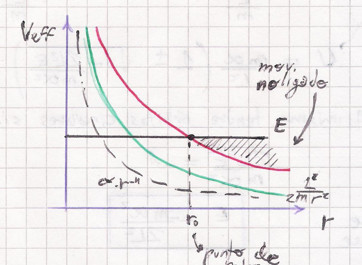
\includegraphics[width=0.4\textwidth]{images/fig_mc_potencialcentral1.jpg}

En el caso de partícula libre, $\alpha=0$, a cierta velocidad se tendrá el siguiente gráfico de potencial. El otro 
gráfico ilustra la posible situación real (en el espacio físico)
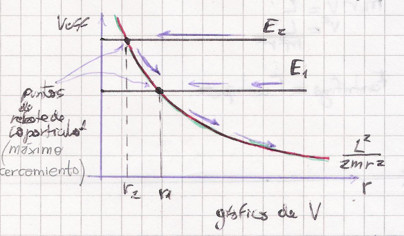
\includegraphics[width=0.4\textwidth]{images/fig_mc_potencialcentral2.jpg}
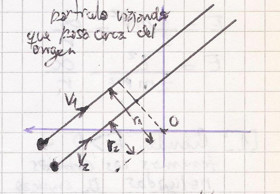
\includegraphics[width=0.4\textwidth]{images/fig_mc_potencialcentral3.jpg}

Finalmente el caso de un potencial atractivo, $\alpha < 0 $ se tienen energias para las cuales el movimiento es ligado.
Cuando existen radios mínimo y máximo se tendrá una órbita como la que se ilustra en el segundo gráfico

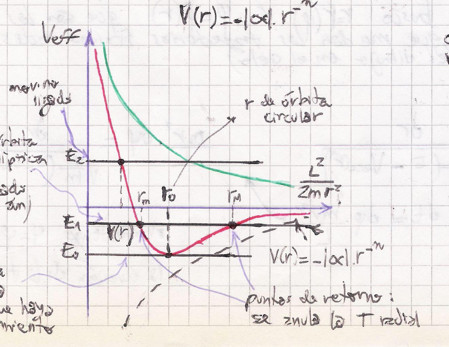
\includegraphics[width=0.4\textwidth]{images/fig_mc_potencialcentral4.jpg}
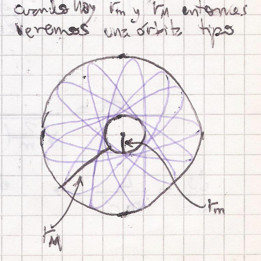
\includegraphics[width=0.4\textwidth]{images/fig_mc_potencialcentral5.jpg}

En los puntos de retorno se anula la energía cinética radial $T$.
El momento angular $L$ es el responsable de que haya satélites orbitando a los planetas; si $L=0$ la partícula pasaría 
por el origen.

En el gráfico bajo estas líneas ilustramos muchas de las características de la física del problema
de fuerzas centrales.

\begin{figure}[!hbt]
	\begin{center}
	\includegraphics[width=0.9\textwidth]{images/fig_mc_potencialcentral.pdf}	 
	\end{center}
	\caption{}
\end{figure} 

\notamargen{Este gráfico hay que tirarlo de inmediato.}

Calculemos ahora los puntos de retorno.
Tomando el cambio de variables $U=1/r$ en la ecuación de la energía es
\[
	\frac{L^2}{2m} U^2 - \alpha U - E = 0,
\]
una cuadrática para $U$ con soluciones
\be
	U = \frac{m\alpha}{L^2}\left( 1 \pm \sqrt{1 + 2L^2E/(m\alpha^2) }\right)
	\label{ec_puntos_retorno_U}
\ee
y entonces
\[
	U_+ = \frac{1}{r_m} \qquad U_- = \frac{1}{r_M}
\]

Si requiereo que $U>0$ en cada caso, necesito $ \sqrt{1 + 2L^2E/(m\alpha^2) } < 1 $ de manera que $ E < 0 $.

Asimismo tendré órbitas circulares si
\[
	\frac{ 2 L^2 E }{ m \alpha^2 } = - 1
\]
lo que significa que 
\[
	E = -\frac{m\alpha^2}{2L^2}.
\]

Puedo calcular el radio de órbita circular haciendco que la fuerza radial se compense exactamente con la fuerza 
centrífuga
\[
	m r v = L
\]
y entonces
\[
	E = \frac{L^2}{2mr^2} - \frac{\alpha}{r}.
\]

Cuando $E>0$ se ve en \eqref{ec_puntos_retorno_U} que se obtienen las órbitas no ligadas; $U_-$ empieza a ser negativa 
y hay que descartarla porque significa un $r_M$ negativo.

Una vez en posesión de $r(t), \phi(t)$ se pueden calcular $r(\phi)$ o $\phi(r)$ que son las funciones que me darán las
trayectorias físicas reales ({\it el dibujo en el cielo}).
Utilizando $d\phi/dt = L/(m r^2 )$ en $dr/dt$ se llega a 
\[
	dt = \frac{dr}{\sqrt{2/m(E-V_{\text{eff}}(r))}}  = \frac{ m r^2 }{ L } d\phi
\]
y ahora se tiene $\phi = \phi(r)$ que es la ecuación de la trayectoria, cuya integral es
\[
	\int_{\phi_0}^{\phi} d\phi = \int_{r_0}^r \frac{L}{mr^2} \frac{dr}{\sqrt{2/m(E-V_{\text{eff}}(r))}}
\]

La ecuación de movimiento para $r$ [¿?]
\[
	m \dtot[2]{r}{t} - \frac{L^2}{mr^3} = -\dtot{V}{r}
\]
y la relación 
\[
	\frac{mr^2}{L} d\phi = dt
\]
permite transformar una derivada temporal en una derivada con respecto al ángulo,
\[
	\dtot{}{t}\left( \phantom{\frac{}{}} \right) = \frac{L}{mr^2} \dtot{}{\phi}\left( \phantom{\frac{}{}} \right)
\]
de modo que la ecuación de arriba se convierte en
\[
	\frac{L}{r^2}\dtot{}{\phi}\left( \frac{L}{mr^2} \dtot{r}{\phi} \right) - \frac{L^2}{mr^3} = -\dtot{V}{r},
\]
es decir en
\[
	-\frac{L^2}{mr^4}\dtot[2]{r}{\phi} - \frac{L^2}{mr^3} = -\dtot{V}{r}.
\]

Proponiendo el cambio de variables $U = 1/r$ se tiene 
\[
	dU = -\frac{1}{r^2} dr,
\]
y entonces
\[
	\dtot{U}{\phi} = -\frac{1}{r^2} \dtot{r}{\phi}.
\]
La ecuación en términos de $U$ luce como
\[
	\dtot[2]{U}{\phi} + U = -\frac{m}{L^2U^2} \: F(1/U),
\]
donde $F(1/U) = dV / dr(U)$.
\notamargen{Esto ilustra un procedimiento elemental y usual en resolución de ecuaciones diferenciales que es el de
cambio de variables. Decir algo al respecto.}

Para el caso de un potencial newtoniano (problema de Kepler) tendremos 
\[
	-\frac{m}{L^2U^2} \: F(1/U) = \frac{\alpha m}{L^2}
\]

% =================================================================================================
\section{Solución a partir de las ecuaciones de Euler-Lagrange}
% =================================================================================================

\[
	m \ddot{r} -\frac{L^2}{m r^3} -\dpar{V}{r}= 0 
\]
\[
	d \phi = \frac{L}{m r^2} dt \qquad \longrightarrow \quad  \dpar{\phi}{r}\dpar{r}{t}  = \frac{L}{m r^2}
\]
\[
	\frac{d}{t}(\dot{r}) = \frac{L}{m r^2} \frac{d}{\phi}(\dot{r})
\]
\[
	m \dtot[2]{r}{t} -\frac{L^2}{m r^3} = -\dpar{V}{r}
\]
\[
	\frac{L}{r^2} \frac{d}{\phi}\left( \dtot{r}{t} \right) -\frac{L^2}{m r^3} = -\dtot{V}{r}
\]
\[
	\frac{L}{r^2} \frac{d}{\phi}\left( \frac{L}{m r^2}\dtot{r}{\phi} \right) -\frac{L^2}{m r^3} = -\dtot{V}{r}
\]
y acá probamos el conveniente cambio de variables
\[
	U = \frac{1}{r} \qquad dU = -\frac{1}{r^2} dr 
	\qquad \dtot{U}{\phi} = -\frac{1}{r^2}\dtot{r}{\phi} = -U^2\dtot{r}{\phi}
\]
\[
	U^2 L \frac{d}{d\phi} \left\{ -\frac{L}{m}\dtot{U}{\phi} \right\} - \frac{L^2}{m r^3} U^3 = F(1/U)
\]
\[
	- \frac{U^2 L^2}{m} \dtot[2]{U}{\phi} - \frac{L^2}{m r^3} U^3 = F(1/U)
\]
\[
	- \frac{U^2 L^2}{m} \left[ \dtot[2]{U}{\phi} + U \right] = F(1/U)
\]
o bien
\[
	\left[ \dtot[2]{U}{\phi} + U \right] = - \frac{F(1/U) m}{U^2 L^2}. 
\]

En el caso del potencial de Kepler será 
\[
	\left[ \dtot[2]{U}{\phi} + U \right] = - \frac{K m}{L^2},
\]
es decir que el miembro derecho es una constante. Sale fácil entonces.

% =================================================================================================
\section{Velocidad areolar}\index{Velocidad areolar--}
% =================================================================================================

\[
	\dot{\phi} = \frac{L}{m r^2}
\]
\begin{figure}[hbt]
	\begin{center}
	\includegraphics[width=0.4\textwidth]{images/fig_mc_velareolar.pdf}	 
	\end{center}
	\caption{}
\end{figure} 
De la figura puede verse que 
\[
	A = \frac{1}{2} r^2 d\phi 
\]
y  entonces
\[
	\dtot{A}{t} = \frac{1}{2} r^2 \dtot{\phi}{t} = \frac{1}{2} r^2 \dot{\phi} = \frac{1}{2}\frac{L}{m} = cte.
\]

% =================================================================================================
\section{Las fuerzas centrales y las leyes de Kepler}
% =================================================================================================

Tenemos 
\[
	\int d\phi = \int \frac{(L/Mr^2)}{\sqrt{ \frac{2}{m}(E - V_{\text{eff}})}} dr	\qquad
	\dtot[2]{U}{\phi} + U  = - \frac{F(1/U) m}{U^2 L^2} \quad U = 1/r
\]
que es simétrica respecto a $\phi$ y $-\phi$. Esto determina una simetría orbital si
tomamos
\[
	U(\phi=0) = U_0 	\qquad		\left. \dtot{U}{\phi} \right|_{\phi=0}= 0
\]
lo cual significa que $U_0$ es un extremo (punto apsidal).

Calculemos ahora el ángulo que recorre una oscilación completa,
\[
	\Delta \phi = 2\int_{r_m}^{r_M} \frac{(L/Mr^2)}{\sqrt{ \frac{2}{m}(E - V_{\text{eff}})}} dr
\]

Si $\Delta \phi = 2 q $ siendo $q= (m/n)\pi $ son $m,n \in \mathbb{Z}$ entonces
\[
	\Delta \phi = 2 \frac{m}{n} \pi 
\]
\[
	\frac{m}{n} = \frac{2\pi}{\Delta \phi}
\]
y esto significaría que la órbita se cierra.

La ecuación a resolver es 
\[
	\dtot[2]{U}{\phi} + \left( U  - \frac{k m}{L^2} \right) = 0.
\]
Si consideramos una nueva variable 
\[
	\beta = U  - \frac{k m}{L^2}
\]
la anterior pasa a 
\[
	\dtot[2]{\beta}{\phi} + \beta = 0
\]
y es fácil ver que la solución es
\[
	\beta = A \cos( \phi -\phi_0 ),
\]
o bien 
\be
	U(\phi) = \frac{km}{L^2} +  A \cos( \phi -\phi_0 ),
	\label{sol_general}
\ee
donde $A,\phi_0$ son constantes. Ahora bien, la expresión \eqref{sol_general} es la solución general,
necesitamos proveer las condiciones iniciales para fijar $ A, \phi_0 $. Propongamos $ \phi_0 = 0 $
punto apsidal.
\notamargen{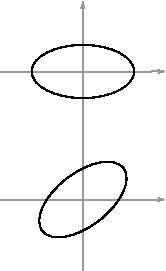
\includegraphics[width=0.3\textwidth]{images/fig_mc_detalle_elipses.pdf}
Eligiendo el punto $\phi_0 =0$ obtenemos una elipse como la de arriba.
}
Luego podemos utilizar $r_m, r_M$ lo cual determina $U_m, U_M$ respectivamente, cuyos valores son 
\[
	U^M_m = \frac{km}{L^2} \left( 1 \pm \sqrt{1 + \frac{2EL^2}{k^2 m} }\right)
\]

y esto nos permite fijar $A$. Incorporando esto en \eqref{sol_general} y recordando que $U(\phi) =1/r$ 
se tiene 
\[
	\frac{1}{r} = \frac{km}{L^2}\left( 1 +  \sqrt{1 + \frac{2EL^2}{k^2 m} } \cos( \phi ) \right),
\]
que no es otra cosa que la ecuación de una elipse en coordenadas polares con origen en un foco.
Veámoslo.

% \[
% 	\frac{1}{r} = \frac{km}{L^2} +  A \cos( \phi -\phi_0 )
% \]
% y habría que usar $r_m, r_M$ para evaluar $A$.

Las elipses verifican 
\[
	\frac{x^2}{a^2} + \frac{y^2}{b^2} = 1	\qquad \sigma^2 = a^2 - b^2
\]
donde $\sigma$ es la semi-distancia focal. Definiendo $ \sigma/a \equiv \varepsilon$ (la excentricidad) 
se puede expresar
\[
	b = a \sqrt{ 1 - \varepsilon^2 }
\]
\notamargen{Falta el sistema de coordenadas en el foco $f'$. Revisar quién es $EL$.}
\begin{figure}[hbt]
	\begin{center}
	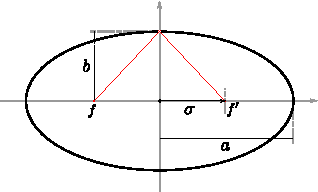
\includegraphics[width=0.4\textwidth]{images/fig_mc_elipse_1.pdf} \hspace*{2em}	 
	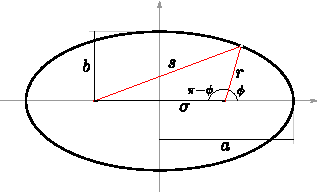
\includegraphics[width=0.4\textwidth]{images/fig_mc_elipse.pdf}	 
	\end{center}
	\caption{}
	\label{fig_mc_elipse}
\end{figure} 

Por otro lado, usando el teorema del coseno para el triángulo definido en la Figura \ref{fig_mc_elipse} es 
\[
	s^2 = (2\sigma)^2 + r^2 - 4\sigma r \cos( \pi - \phi )
\]
y como $s+r$ es la distancia que se mantiene constante e igual, entre otras, a $2a$ se sigue que 
\[
	( 2a -r )^2 = 4\sigma^2 + r^2 + 4\sigma r \cos(\phi)
\]
cuya simplificación conduce a
\[
	\frac{1}{r} = \frac{1 + \varepsilon \cos (\phi)}{a(1-\varepsilon)} = \frac{a}{\phantom{^a}b^2} \left( 1 + 
\varepsilon \cos (\phi) \right)
\]
la cual es la ecuación de una elipse.

\notamargen{Acá hay que hacer un laburo muy importante.}
% \begin{figure}[hbt]
% 	\begin{center}
% 	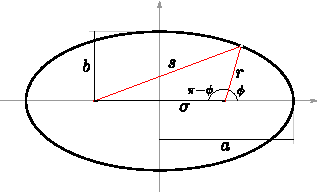
\includegraphics[width=0.4\textwidth]{images/fig_mc_elipse.pdf}	 
% 	\end{center}
% 	\caption{}
% \end{figure} 

Entonces en resumen, las leyes de Kepler son
\begin{enumerate}
 \item Los planetas giran en órbitas elípticas con el Sol en uno de sus focos. Esto es común de los potenciales del 
tipo 
	\[
		V \propto 1/r
	\]
 \item El radio vector recorre áreas iguales en tiempos iguales
	\[
		\delta A = \frac{1}{2} r^2 \delta \phi \quad \longrightarrow \quad \dtot{A}{t} = \frac{r^2}{2} 
\dot{\phi} = \frac{L}{2m} (cte.)
	\]
	Esto es una característica de todo potencial central.
 \item El cubo del semieje mayor de la órbita de un planeta es proporcional al cuadrado del período empleado en 
recorrerla.
	La ecuación anterior, que da la velocidad areolar, se puede integrar como 
	\[
		\int dA  = \frac{L}{2m} \int dt
	\]
	que conduce a 
	\[
		\pi a b = \frac{L}{2m} \tau \qquad \longrightarrow \qquad a = \frac{L\tau}{2\pi b m}, 
	\]
	y luego, como $k m /L ^2 = a/b^2$ llegamos a 
	\[
		a^3 = \frac{k}{m} \frac{1}{4\pi^2} \: \tau^2 = \frac{GM}{4\pi^2} \tau^2
	\]
 y esto es independiente de la masa del planeta.
 
Como $a$ depende de $L$ se tiene que dependiendo de la energía $E$ tendré órbitas como las ilustradas debajo
todas las cuales tienen la misma energía 
\[
	a = \frac{1}{2}(r_M + r_m) = -\frac{k}{2E}
\] 
\notamargen{Esto estaba en la carpeta pero no lo entiendo bien del todo. Tal vez ilustración de la elipse con 
el sistema coordenado en el origen.}
 Para una elipse con el sistema coordenado en el centro se tiene 
 \[
	\frac{1}{r^2} = \frac{1}{b^2}( 1-\varepsilon^2 \cos^2 (\phi) )
 \]
 
 Trabajamos más con la elipse,
 \[
	r_M + r_m = 2a
 \]
 \[
	E = \frac{L^2}{2mr^2} - \frac{k}{r}	\qquad\qquad E - \frac{L^2}{2m} U^2 - kU = 0
 \]
 \[
	\frac{1}{r_{m,M}} = \frac{ \frac{2mkE}{L^2} \mp \sqrt{ \left(\frac{2mkE}{L^2}\right)^2 + \frac{8mE}{L^2} } }{2}
 \]
 \[
	\frac{1}{r_{m,M}} = \frac{mEk}{L^2} \left( 1 \pm \sqrt{1 - \frac{2L^2}{mEk^2}}\right) 
 \]
 y acá constatamos que representa una elipse; es decir que las órbitas son elípticas.
\end{enumerate}

\begin{ejemplo}{\bf Problema 1 de central forces}

Conviene pasarlo a un problema equivalente para una partícula {\it masa reducida} en términos del centro de masa.
\[
	E = \frac M 2 V_{cm}^2 + \frac \mu 2 ( \dot{r}^2 + r^2\dot{\theta}^2 ) + V( r )
\]
\[
	\tau = \frac{2\pi R}{R\dot{\theta}}
\]

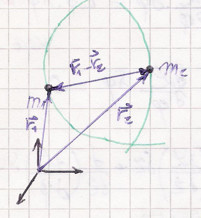
\includegraphics[scale=0.4]{images/fig_mc_central_forces1.jpg}

\[
	E = \frac 1 2 \mu(\dot{r}^2 + r^2\dot{\theta}^2 ) + \frac K r
\]
Al detenerlas,
\[
	E = - \frac K r
\]
y al rearrancar
\[
	E = \frac 1 2 \mu \dot{r}^2 - \frac K r
\]
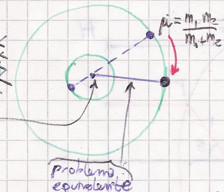
\includegraphics[scale=0.4]{images/fig_mc_central_forces2.jpg}

Para la integración le pongo el signo negativo puesto que corresponde a la situación física correcta
\[
	\dtot{r}{\tau} = -\sqrt{ \frac 2 \mu \left(E + \frac K r \right) }
\]
Integración a ambos miembros lleva a
\[
	\int_0^\tau dt = - \int_R^0 \frac{dr}{ \sqrt{ \frac 2 \mu \left(E + \frac K r \right) } }
\]
o bien a 
\[
	\tau' = \sqrt{\frac{\mu}{2}} \sqrt{\frac{R}{K}} \int_R^0 \sqrt{\frac{r}{R-r}} dr
\]

Con el cambio de variables $U=\sqrt{R-r}$ que lleva al diferencial 
\[
	dU = \frac{-dr}{2\sqrt{R-r}}
\]
la integral resulta en 
\[
  	2 \left( \frac{ \mu R }{ 2K } \right) \int_0^{\sqrt{R}} \sqrt{ R - U^2 } dU =
 	2 \left( \frac{\mu R}{2K}\right) \left( \frac{ U\sqrt{R-U^2} }{2} + \frac{R}{2} 
 	\asen\left( \frac{U}{\sqrt{R}}\right) \right)
\]
que se ha buscado en tablas.
Luego,
\[
	\tau' = \sqrt{ \frac{\mu R}{2K} }\frac{R\pi}{2}
\]
y las ecuaciones de Newton,
\[
	\frac{K}{R^2} = \mu R\dot{\theta}^2 
\]
de la cual se puede despejar $\dot{\theta}$ para obtener
\[
	\tau = 2 \pi R \sqrt{\frac{\mu R}{K}}
\]
de manera que 
\[
	\frac{ \tau }{ \tau' } = 4 \sqrt{ 2 }.
\]
\end{ejemplo}

\begin{ejemplo}{\bf Problema 4 de central forces}

Consideramos un potencial de la forma 
\[
	V(r) = \frac{K}{r^2}
\]
que es un potencial repulsivo puesto que 
\[
	F(r) = -\dpar{V}{r} = \frac{2K}{r^3}
\]
implica que {\it aleja a la partícula}.
Como es central, conserva $ L = m r^2 \dot{\theta} $ se puede escribir la energía como
\[
	E = \frac 1 2 m ( \dot{r}^2 + r^2 \dot{\theta}^2 ) + \frac K {r^2} = \frac{ m \dot{r}^2 }{2} +
	\left( \frac{ \ell }{ 2 m r^2 } + \frac{ K }{ r^2 } \right)
\]

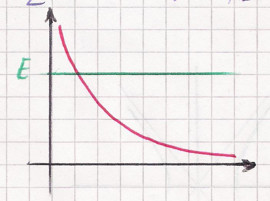
\includegraphics[scale=0.3]{images/fig_mc_potencial_central_4.jpg}

Luego,
\[
	\dot{r} = \sqrt{ \frac{2E}{m} - \frac{2L}{2m^2r^2} - \frac{2K}{mr^2} }
\]
y entonces
\[
	m r^2 \sqrt{ \frac{2E}{m} - \frac{2L}{2m^2r^2} - \frac{2K}{mr^2} } \dtot{\theta}{r} = L
\]
de manera que 
\[
	\int_0^{\theta} d\theta = \frac{L}{\sqrt{2m}} \int_{r_0}^{r} \frac{dr}{r^2( E - L/(2mr^2) - K/r^2 )^{1/2}}
\]

Con el cambio de variables $ U = 1 / r $
\[
	\theta = -\frac{L}{\sqrt{2m}} \int_{1/r_0}^{1/r} \frac{ dU }{ [ E - U^2( L/(2m) + K )]^{1/2} }
\]

Integrada da
\[
	\theta = \frac{L}{m\sqrt{2Km + \frac{L^2}{m^2}}}
	\left( \acos\left[ \frac{ \sqrt{2Km + L^2/(m^2)} }{r_0\sqrt{2E/m}} \right] - 
	\acos\left[ \frac{\sqrt{2Km + L^2/(m^2)}}{r\sqrt{2E/m}}\right] \right).
\]

Tomo $r_0$ punto de retorno
\[
	E = \left( \frac{L^2}{2mr_0^2} + \frac{K}{r_0^2} \right)
\]
y entonces
\[
	r_0 = \sqrt{ \frac L {2mE} + \frac K E }
\]
\[
	\theta = \frac{L}{m\sqrt{2Km + \frac{L^2}{m^2}}} \acos\left(\frac{r_0}{r}\right)
\]
y se puede despejar
\[
	r = \frac{ r_0 }{\cos( \theta m / L \sqrt{ 2 m K + L^2 / m^2 } )}
\]
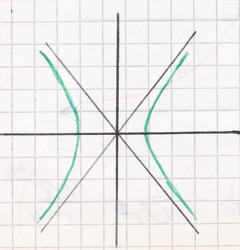
\includegraphics[scale=0.3]{images/fig_mc_potencial_central_4_orbitas.jpg}

Continuamos con el problema [esto sacarlo, je!]

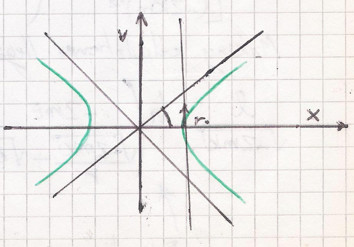
\includegraphics[scale=0.3]{images/fig_mc_potencial_central_5_orbitas.jpg}
\[
	r = \frac{ r_0 }{ \cos( \vp \sqrt{ 2 m^3 K / L^2 + 1 } ) }
\]
\notamargen{Ojo, chequear esta expresión porque en la carpeta está distinta!}

Vemos el comportamiento asintótico, si $ K = 0 $ entonces
\[
	r = \frac{ r_0 }{ \cos \vp }.
\]
Si el potencial es atractivo, por ejemplo $ V(r) = -\frac{K}{r^2}$ entonces se puede escribir 
\[
	E = \frac{1}{2} m \dot{r}^2 + \frac{K'}{r^2},
\]
donde 
\[
	K' = \left( \frac{L^2}{2m} - \frac{K}{} \right).
\]
Entonces la velocidad será 
\[
	\dot{r} = \sqrt{ \frac{2}{m}\left( E - \frac{K'}{r^2} \right) }
\]

A partir de la ecuación para el momento angular, $ m r^2 \dot{\vp} = L $ podemos llegar a la integral para $\vp(r)$ [esto creo que ya se hizo en la 
teoría, en dicho caso citar, sino hacer en detalle]
\[
	\int d\vp = \int \frac{L}{m} \frac{ dr }{ r^2 \sqrt{ \frac{2}{m}\left( E - \frac{K'}{r^2} \right) }}
\]
Con el reemplazo usual $r = 1/U$ se llega a 
\[
	\vp = -L \int \frac{ dU }{ ( 2mE - K'mU^2 )^{1/2}}.
\]

Si $L^2 > 2mK$ es 
\[
	\frac{L^2 - 2mK}{2m} > 0 \qquad K'>0
\]
y tengo un caso similar al anterior (en la página precedente[sic carpeta?]). En cambio si $ L^2 < 2mK $ se tiene $ K' < 0 $.
Usano la ayuda para la integral [refiere al enunciado en la guia?] que se hace entre $r_0$ y algún $r$ final resulta 
\[
	\vp =  \frac{L}{\sqrt{-2mK'}} \log \left( \frac{-2mE}{ \sqrt{ -2mK'/r } + \sqrt{2mE - K'/r^3} }\right)
\]
y esto dice que la partícula cae al origen describiendo una espiral. En el origen es $\dot{\vp} \to \infty$

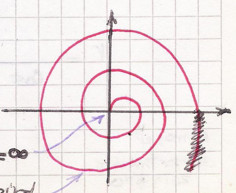
\includegraphics[scale=0.3]{images/fig_mc_potencial_central_6_orbitas.jpg}

Dicho esto, se puede calcular el tiempo que tarda en caer al origen a partir de la ecuación para $\dot{r}$
\[
	-\int_{r_0}^0 \frac{1}{\sqrt{ 2/m ( E - K'/r^2 ) }} = \int_0^{t_f} dt
\]
Como la energía se conserva puede utilizarse su valor inicial, $E=K'/r_0^2$ de modo que el LHS de la ecuación anterior es
\[
	t_f = -\sqrt{ \frac{m}{-2K'} } \int_{r_0}^0 \frac{ r_0 r }{\sqrt{ r_0^2 - r^2 }} = r_0^2 \sqrt{\frac{m}{-2K'}}.
\]
\end{ejemplo}

% =================================================================================================
\section{Teorema del virial}
% =================================================================================================

Se aplica a sistemas de muchas partículas. Defino 
\[
	G \equiv \vb{p}_i \cdot \vb{x}_i
\]
de modo que como $ \dot{\vb{p}}_i = \vb{F}_i $ se tiene 
\[
	\dtot{G}{t} = \dtot{\vb{p}_i}{t} \cdot \vb{x}_i + \vb{p}_i \dtot{\vb{x}_i}{t}
\]
y se puede ver que el último miembro del RHS es $ \vb{p}_i \dot{\vb{x}}_i = m_i v_i^2 = 2T$ donde $T$ es la energía cinética del sistema.
Luego 
\[
	\dtot{G}{t} = \sum_i^N \dtot{\vb{p}_i}{t} \cdot \vb{x}_i + 2 T
\]

Defino el valor medio temporal de una cantidad $A$ según 
\[
	\bar{A} = \lim_{\tau \to \infty} \frac{1}{\tau} \int_0^\tau A(t) dt
\]
[Pasar esto a Apéndice!!].
\[
	\overline{G} = \frac{1}{\tau} \int_0^\tau \dtot{G}{\tau} dt = \overline{ 2 T } + \overline{ \sum_i^N \vb{F}_i \cdot \vb{x}_i }
\]
Pero el integrando en el LHS es un diferencial total, entonces 
\[
	\frac{1}{\tau} \left( G(\tau) - G(0) \right) = \overline{ 2 T } + \overline{ \sum_i^N \vb{F}_i \cdot \vb{x}_i }
\]

Si ahora estoy trabajando con un sistema que realiza un movimiento períódico, entonces en $\tau$ definido como ese período tiene 
\[
	\overline{ 2 T } + \overline{ \sum_i^N \vb{F}_i \cdot \vb{x}_i } = 0
\]
lo cual lleva a el teorema del virial\index{Virial, teorema del}
\[
	\overline{ T }  = - \frac{1}{2} \overline{ \sum_i^N \vb{F}_i \cdot \vb{x}_i }.
\]


% =================================================================================================
\section{Vector de Runge-Lenz}
% =================================================================================================

Para el problema de Kepler también se conserva una cantidad llamada {\it vector de Runge-Lenz} definido como
\[
	\vb{R} = \vb{v} \times \vb{l} - \alpha \frac{\vb{x}}{x}.
\]

Luego, si le tomamos la derivada temporal, resulta
\[
	\dtot{\vb{R}}{t} = \left( \dtot{\vb{v}}{t} \times \vb{l} \right) + \left( \vb{v} \times \dtot{\vb{l}}{t} \right)
	- \alpha\frac{ \vb{v} }{x} + \frac{ \alpha }{x^2} \dtot{x}{t} \vb{x}
\]
donde el último se puede poner en términos de la velocidad si utilizamos la regla de la cadena así
\[
	\dtot{|\vb{x}|}{t} = \dtot{|\vb{x}|}{x_i} \dtot{x_i}{t} = \nabla( |\vb{x}| )\cdot \vb{v} \qquad  \qquad i=1,2,3
\]

Luego, cada componente $i$-ésimo del gradiente de la norma del vector de posición tiene (en coordenadas cartesianas) la 
misma
forma; tomando como ejemplo el $i=1$
\[
	\dtot{|\vb{x}|}{x_1} = \dtot{\sqrt{x_1^2 + x_2^2 + x_3^2}}{x_1} = \frac{x_1}{|\vb{x}|},
\]
de manera que 
\[
	\nabla( |\vb{x}| ) = \frac{\vb{x}}{x} = \hat{x},
\]
el gradiente de la norma del vector es su dirección. Entonces, volviendo a la ecuación original resulta 
\[
	\dtot{\vb{R}}{t} = \left( \dtot{\vb{v}}{t} \times \vb{l} \right) + \left( \vb{v} \times \dtot{\vb{l}}{t} \right)
	- \alpha\frac{ \vb{v} }{x} + \alpha \:\vb{x} \left( \frac{ \pe{x}{v} }{x^3}\right) 
\]

Dado que $\vb{l} = \vb{x} \times m \vb{v}$ el segundo término en la anterior expresión desaparece y nos queda
\[
	\dtot{\vb{R}}{t} = \left( \dtot{\vb{v}}{t} \times [ \vb{x} \times m\vb{v} ] \right) 
	- \alpha\frac{ \vb{v} }{x} + \alpha \:\vb{x} \left( \frac{ \pe{x}{v} }{x^3}\right) 
\]

\notamargen{Aparentemente esto tiene que dar nulo pero no lo estaría viendo.}

\[
	\dtot{\vb{V}}{t} \times ( \vb{x} \times m\vb{v} ) +
	\vb{V} \times \left( \dtot{\vb{r}}{t} \times m\vb{v} + \vb{r} \times m\dtot{\vb{v}}{t} \right)
\]
pero como $\dtot{\vb{r}}{t} \times m\vb{v} = 0$ resulta lo que resulta.
\begin{figure}[hbt]
	\begin{center}
	\includegraphics[width=0.4\textwidth]{images/fig_mc_rungelenz.pdf}	 
	\end{center}
	\caption{}
\end{figure} 

El vector de Runge-Lenz siempre apunta en la misma dirección dada su constancia (ver figura).
\notamargen{Mejorar la figura!}

Escribo $ T = E - V $
\[
	r_{max} m v^2 = 2Er_{max} + 2\alpha
\]
pero 
\[
	r_{max} = \frac{2 E l^2 \alpha}{\alpha^2 m (1-\varepsilon)} = \frac{-1}{\alpha}\frac{b^2 
\alpha}{\alpha^2(1-\varepsilon)}
\]
\[
	r_{max} = - (1+\varepsilon) \alpha
\]

\[
	b^2 = a^2( 1 - \varepsilon^2 )
\]

\begin{ejemplo}{\bfseries Vector de Runge-Lenz en órbitas elípticas}
\notamargen{Este título es provisorio}

Sabemos que el vector de Runge-Lenz tiene la forma 
\[
	\vb{A} = \pv{V}{L} - \alpha \frac{\vb{x}}{x}
\]
y cumple 
\[
	\dtot{A}{t} = 0
\]

Veamos qué expresión tiene el módulo $ A \equiv |\vb{A}| $. Tomando el producto escalar 
\[
	\pe{A}{x} = A r \cos \theta = ( \pv{V}{L} )\cdot \vb{x} - \alpha \frac{\pe{x}{x}}{x}
\]
y reescribiendo (ciclicidad del producto vectorial)
\[
	( \pv{V}{L} )\cdot \vb{x} = \vb{L} \cdot ( \pv{r}{v} ) = \vb{L} \cdot \frac{ \vb{L} }{m} = \frac{L^2}{m}
\]
y entonces
\[
	\alpha r \left( 1 + \frac{A}{\alpha} \cos \theta \right) = \frac{L^2}{m}
\]
pero como $ (1 + \varepsilon \cos \theta ) = p / r $ es la excentricidad se tiene $ A = \varepsilon \alpha $.

\end{ejemplo}

% =================================================================================================
\section{Orbitas de potenciales centrales}
% =================================================================================================

\[
	V(r) = -\frac{\alpha}{r}
\]
\[
	V(r) = \frac{ k r^2 }{2}
\]
Estos dos casos dan órbitas cerradas. Pero hay otros potenciales interesantes.
El potencial de Yukawa
\[
	V(r) = - \frac{\euler^{-\lambda r}}{r^\alpha}
\]
que es aproximadamente como un potencial coulombiano apantallado ($\alpha=1,\lambda=0$).
Otro es el oscilador no armónico\index{Oscilador no armónico}
\[
	V(r) = r^\alpha
\]
Algunos casos se muestran bajo estas líneas

\begin{figure}[hbt]
	\begin{center}
	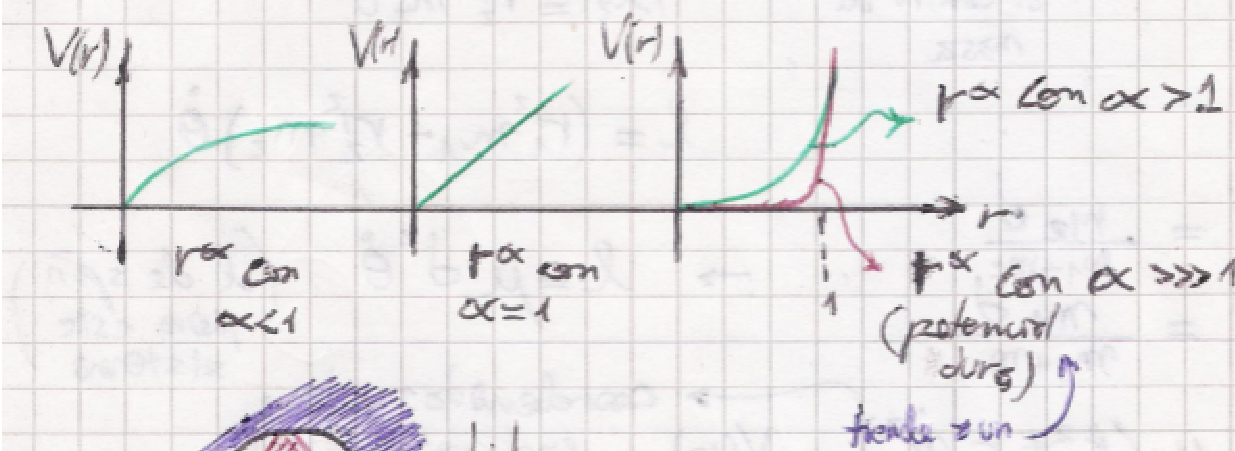
\includegraphics[width=0.6\textwidth]{images/fig_mc_potenciales_otro.pdf}
	\end{center}
	\caption{Algunas curvas de potenciales anarmónicos $ r^\alpha $.}
\end{figure}

Da órbita que no se cierra en un billar elíptico.

\begin{figure}[hbt]
	\begin{center}
	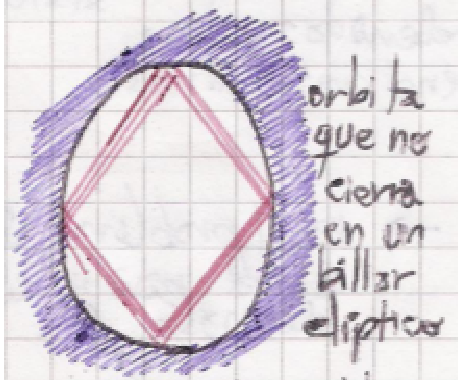
\includegraphics[width=0.4\textwidth]{images/fig_mc_billar.pdf}
	\end{center}
	\caption{.}
\end{figure}

% =================================================================================================
\section{Reducción del problema de dos cuerpos a uno equivalente}
% =================================================================================================

Para dos partículas de masas $ m_1 $ y $ m_2 $ sometidas a una fuerza central 
\[
	\vb{F}_{21} = F(r) \hat{r}_{21} \qquad \qquad F(r) = -\dtot{V(r)}{r}
\]
siendo $x \equiv |\vb{x}_2-\vb{x}_1|$ la distancia relativa.

\begin{figure}[hbt]
	\begin{center}
	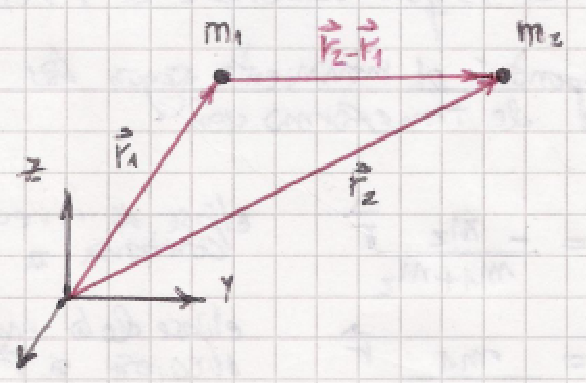
\includegraphics[width=0.4\textwidth]{images/fig_mc_prob_equiv_scheme.pdf}	 
	\end{center}
	\caption{.}
	\label{fig_mc_prob_equiv_scheme}
\end{figure} 

La energía del sistema será de la forma  $ E = T_1 + T_2 + V(r) $ pero se puede expresar según 
$ E = T_{cm} + T_{rel} + V(r) $; es decir separando la energía cinética en el aporte del centro de
masa más un aporte que depende de la distancia relativa entre los cuerpos.
De modo idéntido para el momento angular podemos pasar de $ L_{total} = L_{cm} + L_{spin} $ donde el
momento angular de spin es el referido al movimiento en torno al centro de masas.

\notamargen{Revisar y consolidar toda la notación aquí, que está mezclada.}
Consideramos el siguiente sistema de coordenadas,
\[
	r \equiv | \vb{r}_2 - \vb{r}_1 | \qquad	\qquad  \dot{r} \equiv | \dot{\vb{r}}_2 - \dot{\vb{r}}_1 |
\]
donde el sistema centro de masas es
\[
	\vb{R}_{cm} = \frac{ m_1\vb{r}_1 + m_2\vb{r}_2 }{ m_1 + m_2 }	\qquad 
	M \vb{V}_{cm} =  m_1\vb{v}_1 + m_2\vb{v}_2 
\]
\[
	0 = m_1\vb{r}_1' + m_2\vb{r}_2'
\]
que provocan
\[
	\vb{r}_1' = -\frac{m_2}{m_1}\vb{r}_2' \qquad   \vb{r}_2' = -\frac{m_1}{m_2}\vb{r}_1' 
\]
dando unas $r$ relativas
\be
	\vb{r} = \vb{r}_1' - \vb{r}_2' = -\frac{ m_1 + m_2 }{ m_1 } \vb{r}_2' = -\frac{ m_1 + m_2 }{ m_2 } \vb{r}_1'.
	\label{r_relativas}
\ee

\begin{figure}[hbt]
	\begin{center}
	\includegraphics[width=0.4\textwidth]{images/fig_reduccion.pdf}	 
	\end{center}
	\caption{Sistema coordenado para la reducción del problema de dos cuperpos al de uno equivalente.}
\end{figure} 

Luego, como la energía se conserva (el $V_{cm}=cte.$) podemos escribir
\[
	E = \frac{1}{2} m_1 \dot{\vb{r}}_1^2 + \frac{1}{2} m_2 \dot{\vb{r}}_2^2 + V(r)
\]
\[
	E = \frac{1}{2} m_1 ( \dot{\vb{R}} + \dot{\vb{r}}_1' )^2 + \frac{1}{2} m_2 ( \dot{\vb{R}} + \dot{\vb{r}}_2' )^2 
+ V(r)
\]
\[
	E = \frac{1}{2} m_1 ( {\vb{V}} )^2 +  \frac{1}{2} m_1 ( \dot{\vb{r}}_1' )^2 + 
		\frac{1}{2} m_2 ( {\vb{V}})^2 + \frac{1}{2} m_2 (\dot{\vb{r}}_2' )^2 + V(r)
\]
\[
	E = \frac{1}{2} M {\vb{V}}^2 + \frac{1}{2} \frac{m_2^2}{m_1} \dot{\vb{r}}_2'^2 + \frac{1}{2} m_2 
\dot{\vb{r}}_2'^2 + V(r)
\]
\[
	E = \frac{1}{2} M {\vb{V}}^2 + \frac{1}{2} \frac{m_2 m_1}{M} \dot{\vb{r}}^2 + V(r).
\]

Pero como $E$ y la $\vb{V}$ se conservan, se tiene 
\[
	e \equiv E - \frac{1}{2} M {\vb{V}}^2 =  \frac{1}{2} \mu \dot{\vb{x}}^2 + V(r)
\]
donde $e$ es una cantidad conservada que podemos llamar la energía reducida[?].

Este último $\vb{x}$ es un vector distancia relativa. Es un problema equivalente para la partícula
centro de masas.

\begin{figure}[hbt]
	\begin{center}
	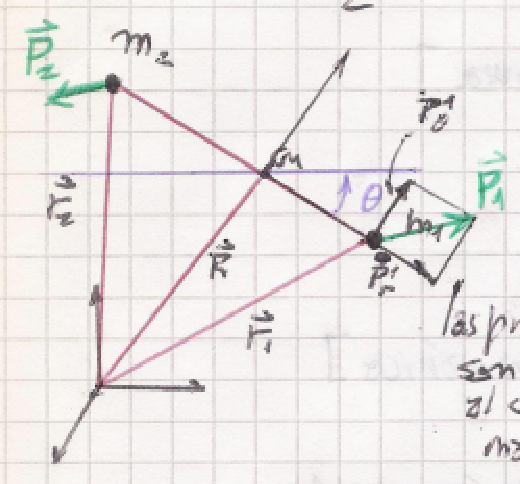
\includegraphics[width=0.4\textwidth]{images/fig_mc_prob_equiv.pdf}	 
	\end{center}
	\caption{.}
	\label{fig_mc_prob_equiv}
\end{figure} 

Podemos considerar ahora los momentos angulares de las partículas respecto de este sistema centro
de masas. Así
\[
	\vb{l}_1' = \vb{x}_1' \times \vb{p}_1 \qquad \qquad  \vb{l}_2' = \vb{x}_2' \times \vb{p}_2'
\]
y sus módulos verifican 
\[
	|\vb{l}_1'| = {x}^{2'}_1 m_1 \dot{\theta} \qquad \qquad  |\vb{l}_2'| = {x}^{2'}_2 m_2 \dot{\theta}
\]
de manera que 
\be
	\ell = ( {x}^{2'}_1 m_1 + {x}^{2'}_2 m_2 ) \dot{\theta} = \mu r^2 \dot{\theta}
	\label{mom_ang_conserv}
\ee
es el momento angular de spín para este sistema. Nótese que a partir de \eqref{r_relativas} se puede
expresar las $x'_i$ ($i=1,2$) en términos de $r$.

Luego, en coordenadas polares en el centro de masa resulta
\[
	e = \frac{1}{2} \mu ( \dot{ r}^2 + r^2\dot{\phi}^2 ) + V(r),
\]
o bien, usando \eqref{mom_ang_conserv},
\[
	e = \frac{1}{2} \mu \dot{ r}^2 + \frac{\ell^2}{2 \mu r^2 } + V(r)
\]
que no es otra cosa que el problema de fuerza central para un cuerpo de masa $\mu$.

Diremos que la {\it distancia relativa} describe una elipse. Las trayectoria reales en el espacio físico
son dos elipses confocales. Por supuesto dejan de cumplirse las leyes de Kepler en este caso.

Si como solución proponemos
\[
	V(r) = -\frac{\alpha}{r}
\]
tendré $ r = r(\phi) $ una elipse, que es lo que describe el $ r $ relativo.
Se descompondrá el movimiento según las ecuaciones de transformación
\[
	\vb{r}_1'= -\frac{m_2}{m_1+m_2} \vb{r} \qquad \text{ Elipse de dirección contraria a $\vb{r}$}
\]
\[
	\vb{r}_2'= \frac{m_1}{m_1+m_2} \vb{r} \qquad \text{ Elipse de dirección igual a $\vb{r}$}	
\]
Tendremos dos elipses confocales como muestra la figura bajo estas líneas 

\begin{figure}[hbt]
	\begin{center}
	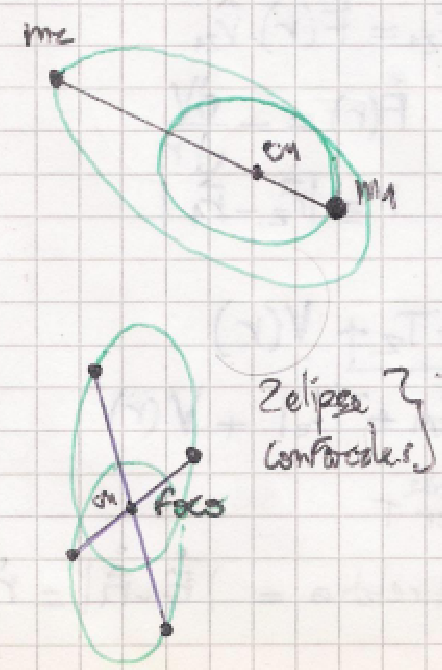
\includegraphics[width=0.4\textwidth]{images/fig_mc_elipses_confocales.pdf}	 
	\end{center}
	\caption{.}
	\label{fig_mc_elipses_confocales}
\end{figure} 

En este caso ya dejan de cumplirse las leyes de Kepler
\[
	\dtot{\mathcal{A}}{t} = \frac{\ell}{2\mu} \qquad a^3 \sim \tau^2 
\]
para la órbita relativa.
\[
	\frac{\pi a b }{\tau}= \frac{\ell}{2\mu} 
\]
\[
	b = \frac{\ell}{\sqrt{\alpha \mu}} a^{1/2} \qquad \frac{a}{b} = \frac{\mu \alpha}{\ell^2}
\]
\[
	\frac{\pi a^{3/2}}{\sqrt{\alpha \mu} \tau} = \frac{1}{2\mu}
\]
y entonces ahora se ve que no es independiente de las masas y no se puede simplificar $\sqrt{\mu\alpha}$ con
$\mu$ como ocurría en un movimiento elíptico tradicional (bajo potencial gravitatorio).
Entonces no es válida la ley de Kepler.
% =================================================================================================
\section{Dispersión}
% =================================================================================================

Consideramos la dispersión de un haz de partículas de cierta energía cinética por un centro dispersor,
ver ilustración.

\begin{figure}[htb]
	\begin{center}
	\includegraphics[width=0.5\textwidth]{images/fig_mc_dispersion1.pdf}	 
	\end{center}
	\caption{}
\end{figure} 
\[
	d\sigma = \frac{dN}{n}
\]
donde $dN$ es el número de partículas dispersadas entre $\chi$ y $\chi + d\chi$ y $n$ es el número de
partículas emitidas por tiempo y por área. De esta forma $d\sigma$ tiene unidades de área.

Consideramos $d$ centro dispersor con simetría esférica (cilíndrica basta).
Usamos como suposiciones que todo lo que emerge entre $\rho + d\rho$ - $\rho$  es dispersado entre
$\chi + d\chi$ - $\chi$, y que se conservan tanto $E$ como \vb{L}.

\begin{figure}[htb]
	\begin{center}
	\includegraphics[width=0.5\textwidth]{images/fig_mc_dispersion2.pdf}	 
	\end{center}
	\caption{}
\end{figure}

El anillo se dispersa en un sector esférico. Entonces podemos establecer las siguientes conclusiones
para el anillo entre $\rho + d\rho$ - $\rho$, a saber
\[
	A =  \pi ( (\rho + d\rho)^2 - \rho^2 ) \qquad \longrightarrow A \approx 2 \pi \rho \: d\rho,
\]
entonces
\[
	d\sigma = \frac{  2 \pi \rho \: d\rho I}{I}
\]
donde $\rho$ es el parámetro de impacto y $I$ el número de partículas por unidad de tiempo y área.
Finalmente
\[
	d\sigma =  2 \pi \rho(\chi) \left| \dtot{\rho}{\chi} \right| d\chi
\]

Como se conservan la energía y el momento angular
\[
	E = \frac{1}{2} m V_\infty^2 \qquad L = m \rho V_\infty^2 
\]
\begin{figure}[htb]
	\begin{center}
	\includegraphics[width=0.5\textwidth]{images/fig_mc_dispersion3.pdf}	 
	\end{center}
	\caption{}
\end{figure}
En general se desconoce $V(r)$.

Se puede calcular el ángulo $\varphi_0$ de acuerdo a 
\[
	\chi = \pi - 2\varphi_0,
\]
donde
\[
	\varphi_0 = \int_{r_m}^{\infty} \frac{L/mr^2}{\sqrt{\frac{2}{m}(E - V_{\text{eff}})}} dr
\]
\[
	\chi = \pi - 2 \varphi_0 (\rho)
\]
e invertimos desde la última ecuación.

Veamos el caso de una esfera maciza. En general los cuerpos duros equivalen a un potencial del tipo
\[
	V = \begin{cases}
	     \infty \qquad \textrm{cuerpo}\\
	     \;0 \qquad \; \textrm{fuera} \\
	    \end{cases}
\]
\begin{figure}[htb]
	\begin{center}
	\includegraphics[width=0.5\textwidth]{images/fig_mc_dispersion4.pdf}	 
	\end{center}
	\caption{}
\end{figure}
\[
	\chi = \pi - 2\varphi_0
\]
\[
	\sin(\varphi_0) = \frac{\rho}{a} \qquad d\rho = -a \frac{1}{2}\cos \left(\frac{\pi-\chi}{2}\right)
\]
y entonces 
\[
	d\sigma = 2\pi a^2 \sin\left(\frac{\pi-\chi}{2}\right) \frac{1}{2}\cos\left(\frac{\pi-\chi}{2}\right) d\chi
\]
\[
	d\sigma = \frac{\pi}{2} a^2 \sin( \pi-\chi) d\chi = \frac{\pi}{2} a^2 \sin( \chi) d\chi
\]
y como hay que integrar $\chi$ de 0 a $\pi$
\[
	\int_0^\pi \frac{\pi}{2} a^2 \sin( \chi) d\chi = \pi a^2
\]
\[
	\sigma = \pi a^2
\]
En el caso de los cuerpos duros la sección eficaz es la sombra de los mismos.
\notamargen{Sobre el ángulo sólido
\[
\Omega = \textrm{Area}/r^2
\]
\[
d\Omega = 2 \pi \sin( \chi ) d\chi 
\]
\[
\Omega = 4 \pi 
\]
para la esfera.
}


% =================================================================================================
\section{Dispersión por dos cuerpos}
% =================================================================================================

Consideramos el caso de un cuerpo que se fracciona en dos (creo?)
\begin{figure}[htb]
	\begin{center}
	\includegraphics[width=0.5\textwidth]{images/fig_mc_disp2body1.pdf}	 
	\end{center}
	\caption{}
\end{figure} 
Desde el centro de masa
\[
	\vb{P}_1 + \vb{P}_2 = 0
\]
\[
	m_1 \vb{v}_1 + m_2 \vb{v}_2 = 0
\]
definimos una velocidad relativa
\[
	\vb{v} \equiv \vb{v}_2  - \vb{v}_1 = \vb{v}_2 \left( \frac{ m_1 + m_2 }{ m_1 }\right) .
\]
\begin{figure}[htb]
	\begin{center}
	\includegraphics[width=0.5\textwidth]{images/fig_mc_disp2body2.pdf}	 
	\end{center}
	\caption{}
\end{figure} 
Con respecto a la energía,
\[
	\frac{1}{2} M \vb{V}_{cm}^2 + e_{int} = \frac{1}{2} m_1 \vb{v}_1^2 + \frac{1}{2} m_2 \vb{v}_2^2
						+ e_{int 1 } + e_{int 2} + \frac{1}{2} M \vb{V}_{cm}^2
\]
\[
	\frac{1}{2} m_1 \vb{v}_1^2 + \frac{1}{2} m_2 \vb{v}_2^2 = e_{int} - e_{int 1 } - e_{int 2} = \Delta e
\]
y pasando todo en términos de la velocidad relativa
\[
	 \frac{1}{2} \frac{m1 m2}{ m_1 + m_2 } v = \Delta e
\]
entonces 
\[
	v = \sqrt{\frac{ 2 \Delta e}{ \mu } }.
\]
\begin{figure}[htb]
	\begin{center}
	\includegraphics[width=0.5\textwidth]{images/fig_mc_disp2body3.pdf}	 
	\end{center}
	\caption{}
\end{figure} 

El problema es evidentemente plano.
\[
	\vb{V}_1^L =  \vb{V}_{cm} + \vb{V}_1' \qquad \longrightarrow \quad ( \vb{V}_1^L - \vb{V}_{cm} ) = \vb{V}_1'
\]
\[
	{V_1^L}^2 - V_{cm} - 2 {\vb{V}_1^L}^2 \vb{V}_{cm} = V_1^2
\]
\[
	{V_{1x}^L}^2 + {V_{1y}^L}^2 - V_{cm} - 2 {V_{1x}^L}^2 V_{cm} = V_1^2
\]
\[
	( V_{1x}^L  - V_{cm} )^2 + {V_{1y}^L}^2 = V_1^2
\]
que es una circunferencia.
\[
	\tan(\theta) = \frac{V_1 \sin(\chi) }{ V_{cm} + V_1 \cos(\chi) }
\]
\begin{figure}[htb]
	\begin{center}
	\includegraphics[width=0.45\textwidth]{images/fig_mc_disp2body4a.pdf}	 
	\includegraphics[width=0.45\textwidth]{images/fig_mc_disp2body4b.pdf}
	\end{center}
	\caption{}
\end{figure} 

Esto tiene dos raíces $\chi_{1,2}$ si $ V_{cm} > V_1$. 

Si $ V_{cm} > V_1$ hay una sola $V$ de las partículas.

Si $ V_{cm} < V_1$ hay partículas emitidas hacia atrás vistas desde L.

Si pensamos en una distribución isótropa de partículas, desde el centro de masa
\[
	e = \frac{1}{2} m_1 V_{1}^2
\]
\[
	V_L^2 = V_1^2 + V_{cm}^2 - 2 V_1 V_{cm} \cos( \pi -\chi )
\]
a iguales $V_1,V_{cm}$ se tienen variables $V_L, \chi$, entonces
\[
	dV_L^2 = - 2 V_1 V_{cm} \sin(\chi) d\chi
\]
\[
	\frac{dV_L^2}{2 V_1 V_{cm}} = \sin( \chi) d\chi 
\]
\[
	d\sigma = 2 \pi \rho |\dtot{\rho}{\chi}| d\chi 
\]
\[
	d\Omega = 2 \pi \sin( \chi ) d\chi 
\]
\[
	\frac{d\Omega}{4\pi} = \frac{1}{2} \sin( \chi ) d\chi 
\]
\[
	\frac{d\Omega}{4\pi} =  \frac{d (V_L^2) }{4 V_1 V_{cm}} = \frac{1}{2} \frac{d ( 1/2 m_1 V_L^2) }{m_1 V_1 V_{cm}} 
\]

% =================================================================================================
\section{Scattering}
% =================================================================================================

Tenemos dos suposiciones básicas:
	\begin{itemize}
		\item Interacción elástica.
		\item Conservación de energía y de momento.
	\end{itemize}

\begin{figure}[htb]
	\begin{center}
	\includegraphics[width=0.5\textwidth]{images/fig_mc_scatt1.pdf}	 
	\end{center}
	\caption{}
\end{figure} 	
	
Desde el centro de masa se tienen:
\[
	\vb{P} = \vb{P}_1 + \vb{P}_2 = 0	\qquad		\vb{r} \equiv \vb{r}_2 + \vb{r}_1
	\qquad		\vb{V} \equiv \vb{V}_2 - \vb{V}_1
\]
donde los últimos son las posiciones y velocidades relativas.
\[
	E = \frac{1}{2} M \vb{V}_{cm}^2 + \frac{1}{2} \mu \vb{V}^2 + V(r)
\]
\[
	m_1 \vb{V}_1 + m_2 \vb{V}_2 = 0 \qquad m_1 \vb{V}_1 = -\frac{m_2}{m_1} \vb{V}_2.
\]
\begin{figure}[htb]
	\begin{center}
	\includegraphics[width=0.7\textwidth]{images/fig_mc_scatt2.pdf}	 
	\end{center}
	\caption{}
\end{figure} 
En términos de las velocidades relativas
\[
	\vb{V}_2 = \frac{m_1}{m_1 + m_2} \vb{V} \qquad \vb{V}_1 = -\frac{m_2}{m_1 + m_2} \vb{V}
\]
Se puede escribir la energía cinética del siguiente modo
\[
	T = \frac{1}{2} m_1 \vb{V}_{1-in}^2 + \frac{1}{2} m_2 \vb{V}_{2-in}^2 =
	\frac{1}{2} M \vb{V}_{cm}^2 + \frac{1}{2} m_1 \vb{V}_{1-cm}^2 + \frac{1}{2} m_2 \vb{V}_{2-cm}^2 
\]
\[
	T - \frac{1}{2} M \vb{V}_{cm}^2 \equiv t = \frac{1}{2} \frac{m_1 m_2}{m_1 + m_2} \vb{V}^2 =
							\frac{1}{2} \mu \vb{V}^2
\]

\[
	\vb{V}_1^L = \vb{V}_{cm} - \frac{m_2}{M} \vb{V}	\qquad \vb{V}_2^L = \vb{V}_{cm} - \frac{m_1}{M} \vb{V}
\]

\[
	\vb{p}_1^L = m_1 \vb{V}_{cm} - \mu \vb{V} = m_1 \frac{\vb{P}}{M} - \mu \vb{V}
\]
\[
	\vb{p}_2^L = m_2 \vb{V}_{cm} + \mu \vb{V} = m_2 \frac{\vb{P}}{M} + \mu \vb{V}
\]
\begin{figure}[htb]
	\begin{center}
	\includegraphics[width=0.35\textwidth]{images/fig_mc_scatttriangle.pdf}	 
	\end{center}
	\caption{}
\end{figure} 
Donde 
\[
	\vb{V}_{cm} + \vb{V}_1 = \vb{V}_1^L
\]
\[
	\vb{p}_2^L = \frac{m_2}{M} \vb{P} + \mu \vb{V}\hat{n}		\qquad	 \vb{p}_1^L = \frac{m_1}{M} \vb{P} - \mu \vb{V}\hat{n}
\]
\[
	\frac{m_2}{M} \vb{P} + \frac{m_1}{M} \vb{P} = \vb{P} = \vb{p}_2^L + \vb{p}_1^L
\]
\[
	\tan(\theta_2) = \frac{P_1 \sin(\chi)}{ (m_2/M) P + P_1\cos(\chi)}
\]

% =================================================================================================
\section{Dispersión por potenciales infinitos}
% =================================================================================================

La idea es que sabiendo $\rho$ (parámetro de impacto) quiero saber qué ángulo $\chi$ se desvían las
partículas incidentes.
\begin{figure}[htb]
	\begin{center}
	\includegraphics[width=0.7\textwidth]{images/fig_mc_potinf.pdf}	 
	\end{center}
	\caption{}
\end{figure} 
\[
	\phi_0 + \alpha = \frac{\pi}{2}		\qquad		2 \phi_0 + \alpha + \beta = \pi
	\qquad \phi_0 + \beta = \frac{\pi}{2}
\]
\[
	\alpha = \beta		\qquad 		2\alpha = 2\beta = \chi
\]
\[
	\dtot{\rho}{z} = \tan \left(\beta \right) = \tan\left(\frac{\chi}{2}\right)
\]
\[
	\tan\left(\frac{\chi}{2}\right) = \dtot{\rho}{z} = \frac{ d\rho/dz }{ dz/d\theta }
\]
con $\theta$ variable paramétrica. Donde $\rho = \rho(z)$ es la función que da la curva roja (el perfil
del cuerpo dispersor).



% =================================================================================================

% \bibliographystyle{CBFT-apa-good}	% (uses file "apa-good.bst")
% \bibliography{CBFT.Referencias} % La base de datos bibliográfica

\end{document}
